\chapter{Hierarchical Clustering}


\section{Learning Objectives}

\begin{itemize}

\item Understand hierarchical clustering algorithm

\item Implement the algorithm
  
\item Learn the binary tree and its properties

\item Use the tree's properties to gain insight of data
  
\end{itemize}

\section{Limitations of the {\it k-mean} Algorithm}

The {\it k-mean} clustering algorithm has third major problems: (1)
There is no obvious reason to select a particular value of $k$.
Figure~\ref{figure:kmean:distances} shows the distances for different
values of $k$. There are 10 clusters and the clusters do not overlap
({\tt -t} not used) but the smallest distance occurs when $k$ is
13. (2) The algorithm is non-deterministic and it is often necessary
running the same program multiple times.
Figure~\ref{figure:kmean:distances} (a) shows that the distances may
vary substantially even for the same value of $k$.  (3) For a given
cluster, there is immediately answer which cluster is closest.  It is
possible to calculate the distances of centroids but this requires
additional calculation.  (4) The {\it k-mean} algorithm assignments
{\it all} data points to one of the $k$ clusters in the very first
step.  Then the algorithm adjusts the clusters by finding closest
centroid from each data point. Because the initial assignments have
direct impacts on the final results, the program needs to run multiple
times for getter better results.  {\it Hierarchical clustering} is a
method that does not have these problems\footnote{Hierarchical
  clustering has some other problems, to be discussed later.}.

\index{binary tree}
\index{binary tree!child}

\section{Example of 
Hierarchical clustering}

Hierarchical clustering iteratively finds the closet pair of data
points, clusters, or data point and cluster. The algorithm makes the
pair two {\it children} by a {\it binary tree}.  The binary tree
becomes a new cluster.  The algorithm continues until only one binary
tree is left.  Hierarchical clustering calls it {\it dendrogram}, instead
of {\it binary tree}.

Before formally describing the algorithm, let us go through several
examples.  The simplest case is when there is only one data point but
it is not very meaningful. Thus, let us start with two data points.

\begin{table}[h]
\begin{tt}
\begin{tabular}{|r|rr|} \hline
{\bf index} &  {\bf x} & {\bf y} \\ \hline
0 &  -66  &  45 \\
1 & 95  &  -84 \\ \hline
\end{tabular}
\end{tt}
\end{table}

They are the two children of a binary tree:

\begin{figure}[h] \centering
{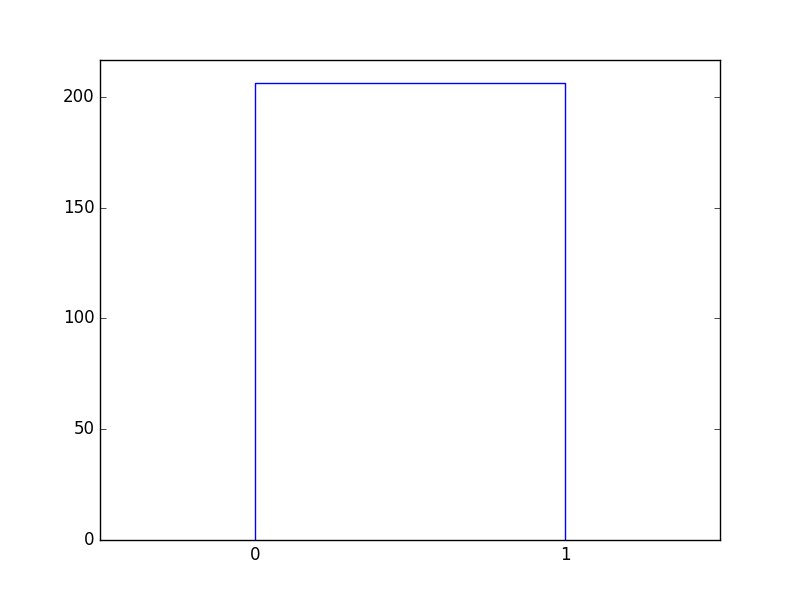
\includegraphics[width=5in]{\hierpath/figures/cluster2.png}}
\caption{Two data points are the two children of a binary tree. }
\end{figure}

Next, we consider the case when there are four data points:

\begin{table}[h]
\begin{tt}
\begin{tabular}{|r|rr|} \hline
{\bf index} &  {\bf x} & {\bf y} \\ \hline
0 &  -66  &  45 \\
1 & 95  &  -84 \\
2 & -35  &  -70 \\
3 & 26  &  94 \\ \hline
\end{tabular}
\end{tt}
\end{table}


Table~\ref{table:hierarchical:distance4points} shows the distance
between each pair of data points.  The distance of $(x_a, y_a)$ and
$(x_b, y_b)$ is $\sqrt{(x_a - x_b)^2 + (y_a - y_b)^2}$. Since we care
about the order, it is not necessary to take the square root.
The
table shows ${(x_a - x_b)^2 + (y_a - y_b)^2}$:
Obviously, this table is symmetric because the distance between $(x_a,
y_a)$ and $(x_b, y_b)$ is the same as distance between $(x_b, y_b)$
and $(x_a, y_a)$. The values along the diagnoal are always zero
because the distance of each point and itself is zero.

\begin{table}
  \begin{tt}
\begin{tabular}{|r|rrrr|}  \hline
& 0 & 1 & 2 & 3  \\ \hline

0 & 0& 42562& 14186& 10865\\
1 & 42562& 0& 17096& 36445\\
2 & 14186& 17096& 0& 30617\\
3 & 10865& 36445& 30617& 0\\ \hline
\end{tabular}
  \end{tt}
  \caption{Distances of pairs of data points.}
  \label{table:hierarchical:distance4points}
\end{table}

The shortest distance (10865) occurs between $(x_0, y_0)$ and $(x_3,
y_3)$.  They are the first pair to be put into the same cluster.
Figure~\ref{fig:hierarchical:cluster4} shows 
the cluster of the four data points. Points 0 and 3 are the two
children of the same parent node. 

\begin{figure}[h] \centering
{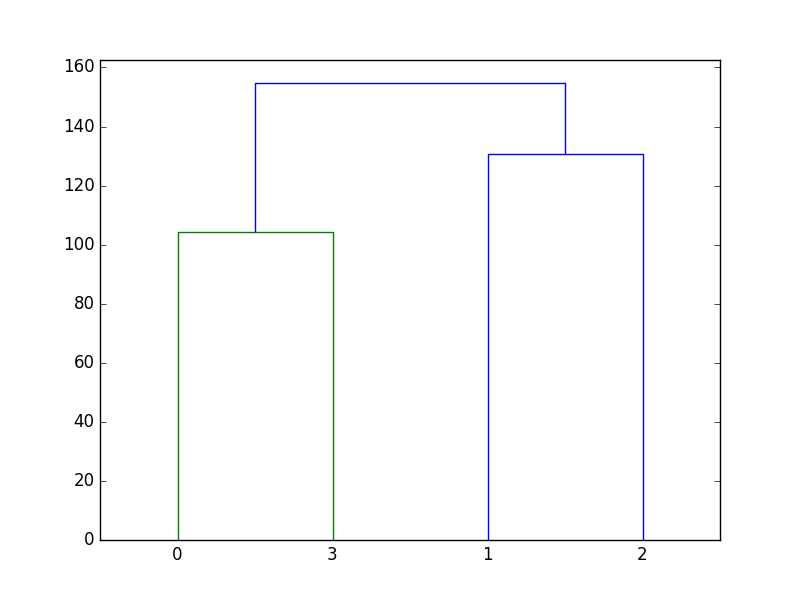
\includegraphics[width=5in]{\hierpath/figures/cluster4.png}}
\caption{Clusters of four data points.
Do not worry about the colors, nor the numbers along the vertical
axis. Pay attention to the shape only.
}
\label{fig:hierarchical:cluster4}
\end{figure}

How do we represent the cluster that includes points 0 and 3?  There
are several different commonly used representations.  This example
uses the {\it centroid}: a cluster is represented by the centroid of
the data points in the cluster.  The cluster that contains $(x_0,
y_0)$ and $(x_3, y_3)$ is represented by $(\frac{-66+26}{2},
\frac{45+94}{2}) = (-20, 69.5)$.  This cluster is marked as $(x_0,
y_0)$ and $(x_3, y_3)$ no longer exists.  We can recompute the
distances among the pairs of points:


\begin{table}
  \begin{tt}
\begin{tabular}{|r|rrr|}  \hline
& 0 & 1 & 2   \\ \hline

0 & 0.0 & 36787.25 & 19685.25 \\
1 & 36787.25 & 0 & 17096 \\
2 & 19685.25 & 17096 & 0 \\ \hline
\end{tabular}
  \end{tt}
  \caption{Distances of one cluster and two  data points.}
  \label{table:hierarchical:distance3}
\end{table}

Now, the shortest distance (17096) occurs between $(x_1, y_1)$ and
$(x_2, y_2)$.  These two data points are the two children of a node.
At this moment, there are only two clusters and they are the children
of a binary tree node.  The final result is shown in
Figur~\ref{fig:hierarchical:cluster4}.

\clearpage

% \begin{figure}[h] \centering
% {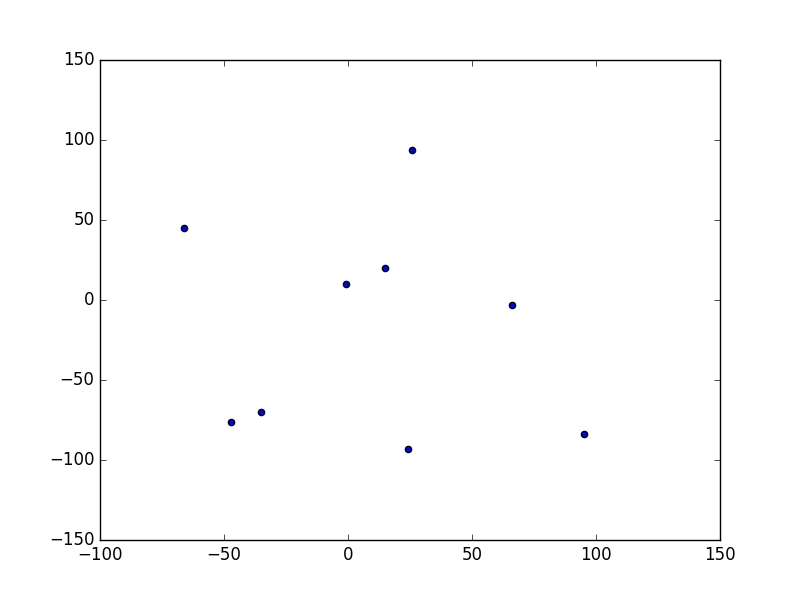
\includegraphics[width=3in]{\hierpath/figures/example1.png}}
% \caption{Locations of nine data points. }
% \end{figure}

These are the locations of the data points:

\hspace{0.1in}
\begin{tt}
\begin{tabular}{|r|rr|} \hline
{\bf index} &  {\bf x} & {\bf y} \\ \hline
0 &  -66  &  45 \\
1 & 95  &  -84 \\
2 & -35  &  -70 \\
3 & 26  &  94 \\
4 & 15  &  20 \\
5 & 66  &  -3 \\
6 & -47  &  -76 \\
7 & 24  &  -93 \\
8 & -1  &  10 \\ \hline
\end{tabular}
\end{tt}
\hspace{0.1in}

  \hspace{0.1in}
  \begin{tt}
\begin{tabular}{|r|rrrrrrrrr|}  \hline
& 0 & 1 & 2 & 3 & 4 & 5 & 6 & 7 & 8 \\ \hline

  0 &0 & 42562 & 14186 & 10865 & 7186 & 19728 & 15002 & 27144 & 5450\\

1 &42562 & 0 & 17096 & 36445 & 17216 & 7402 & 20228 & 5122 & 18052\\

2 &14186 & 17096 & 0 & 30617 & 10600 & 14690 & 180 & 4010 & 7556\\

3 &10865 & 36445 & 30617 & 0 & 5597 & 11009 & 34229 & 34973 & 7785\\

4 &7186 & 17216 & 10600 & 5597 & 0 & 3130 & 13060 & 12850 & 356\\

5 &19728 & 7402 & 14690 & 11009 & 3130 & 0 & 18098 & 9864 & 4658\\

6 &15002 & 20228 & 180 & 34229 & 13060 & 18098 & 0 & 5330 & 9512\\

7 &27144 & 5122 & 4010 & 34973 & 12850 & 9864 & 5330 & 0 & 11234\\

8 &5450 & 18052 & 7556 & 7785 & 356 & 4658 & 9512 & 11234 &
0 \\ \hline
\end{tabular}
\end{tt}
\hspace{0.1in}

Obviously, this table is symmetric because the distance between $(x_a,
y_a)$ and $(x_b, y_b)$ is the same as distance between $(x_b, y_b)$
and $(x_a, y_a)$. The values along the diagnoal are always zero
because the distance of each point and itself is zero.

The shortest distance (180) occurs between $(x_2, y_2)$ and $(x_6,
y_6)$.  They are the first pair to be put into the same cluster.



The second
shortest distance (356) occurs between $(x_4, y_4)$ and
$(x_8, y_8)$.


% a good example in
% http://www.econ.upf.edu/~michael/stanford/maeb7.pdf


% how to plot tree: https://plot.ly/python/tree-plots/
% https://joernhees.de/blog/2015/08/26/scipy-hierarchical-clustering-and-dendrogram-tutorial/
